\chapter{Waves propagations in 3D}
\label{s:laplace3D}
%
\section{General}
%
In this chapter the 3D case will be discussed, looking for
a method to solve the BEM using only the information about
the free surface.
%
This case is our main objective in order to can setup 6-DOF
seakeeping simulations.
%
\section{Incident waves}
%
We can rewrite the sea waves system outside from our
computational domain $\Omega$
%
\begin{eqnarray}
	\label{eq:laplace3D:incident_waves}
	\begin{array}{rcl}
	z(x,y,t) & = & \dsty{\sum_{j=1}^{n_{waves}}} a_j \sin\left(k_j \left(x \cos(\beta) + y \sin(\beta)\right) - \omega_j t + \delta_j \right)
	\\
	v_z(x,y,t) & = & \dsty{\sum_{j=1}^{n_{waves}}} - a_j \omega_j \cos\left(k_j \left(x \cos(\beta) + y \sin(\beta)\right) - \omega_j t + \delta_j \right)
	\\
	\phi(x,z,t) & = & \dsty{\sum_{j=1}^{n_{waves}}} - \frac{a_j \omega_j}{k_j}
	                \cos\left(k_j \left(x \cos(\beta) + y \sin(\beta)\right) - \omega_j t + \delta_j \right)
	                \exp\left(k_j z\right)
	\\
	k_j & = & \dsty{\frac{\omega_j^2}{g}}
	\end{array}
\end{eqnarray}
%
Where $\beta$ is the heading angle, being 0 for stern waves. For
this wave system still being valid the phase velocity from the
equation \ref{eq:laplace2D:c_deep}. The purposed potential is
compatible with the Laplace equation
\ref{eq:governing_equations:laplace} as well.
%
\section{BEM applied to Laplace 3D problem}
\label{ss:laplace3D:bem}
%
\subsection{Computational domain}
\label{sss:laplace3D:computational_domain}
%
We have a domain similar to the shown in the figure
\ref{fig:ss:laplace2D:bem}, but in this case 2 more boundaries
must be considered in the missed direction, that we will call
$\partial \Omega_{Front}$ and $\partial \Omega_{Back}$. As in
the 2D case we will apply the reciprocal relation
%
\begin{eqnarray}
	\label{eq:laplace3D:reciprocal_relation}
	\lambda(X, Y, Z) \phi(X, Y, Z; t) = \int_{\partial \Omega}
	\phi(x, y, z; t) \frac{\partial G(x, y, z, X, Y, Z)}{\partial \bs{n}(x, y, z)} -
	G(x, y, z, X, Y, Z) \frac{\partial \phi(x, y, z; t)}{\partial \bs{n}(x, y, z)}
	\mbox{d} s(x, y, z)
\end{eqnarray}
%
We are focused into compute the gradient of the velocity
potential along the free surface knowing the velocity
potential value in each point one. Let we define the
function $H(x,y,z,X,Y,Z)$ again
%
\begin{eqnarray*}
H(x, y, z, X, Y, Z) = \frac{\partial G(x, y, z, X, Y, Z)}{\partial \bs{n}(x, y, z)}
\end{eqnarray*}
%
As in the Laplace equation for the 2D case, described in the
chapter \ref{s:laplace2D}, we want to expand the domain $\Omega$
such that all the boundaries except the free surface will the
infinity far, adding the boundary $\partial \Omega_{FS,I}$, where
we know the velocity potential and their gradient from
\ref{eq:laplace3D:incident_waves}. In the figure
\ref{fig:ss:laplace3D:bem} a schematic view of the expanded
domain can be seen.\rc
%
The main advantage is that, as happens with the Inlet and the
Outlet, we know all the needed data about the velocity potential,
so we can significantly reduce the linear system matrix dimensions,
and as happens with the bottom, the geometry is so quite similar
to the $\Omega_{FS}$ one, so no additional discretization or memory
storage is needed.\rc
%
This trick will only works if the Green's function $G(x,y,z,X,Y,Z)$,
and their gradient $H(x,y,z,X,Y,Z)$, goes to zero as $(x,y,z)$ goes
to infinite. In 3D Laplace problems we can use the following Green's
function:
%
\begin{eqnarray}
	\label{eq:laplace3D:g}
	G(x,y,z,X,Y,Z) = & \dsty{\frac{1}{\sqrt{\left(x - X\right)^2 + \left(y - Y\right)^2 + \left(z - Z\right)^2}}}
	\\
	\label{eq:laplace3D:h}
	H(x,y,z,X,Y,Z) = & - \dsty{\frac{\left( x - X, y - Y, z - Z \right)}{\left(\left(x - X\right)^2 + \left(y - Y\right)^2 + \left(z - Z\right)^2\right)^{3/2}}}
\end{eqnarray}
%
That in the limit
%
\begin{eqnarray}
	\label{eq:laplace3D:limit_g}
	\lim_{(x-X)^2 + (y-Y)^2 + (z-Z)^2 \to \infty} G(x,y,z,X,Y,Z) = & 0
	\\
	\label{eq:laplace3D:limit_h}
	\lim_{(x-X)^2 + (y-Y)^2 + (z-Z)^2 \to \infty} H(x,y,z,X,Y,Z) = & 0
\end{eqnarray}
%
So in this case, if the potential of the incidents waves is
a good function along all the free surface we can move from
the domain shown in the figure \ref{fig:ss:laplace2D:bem} to
the shown in the figure \ref{fig:ss:laplace3D:bem}, due to
along the other boundaries the Green's functions $G(x,y,z,X,Y,Z)$
and $H(x,y,z,X,Y,Z)$ are nulls, not computing in the equation
\ref{eq:laplace2D:reciprocal_relation}.
%
\begin{figure}[ht!]
  \centering
  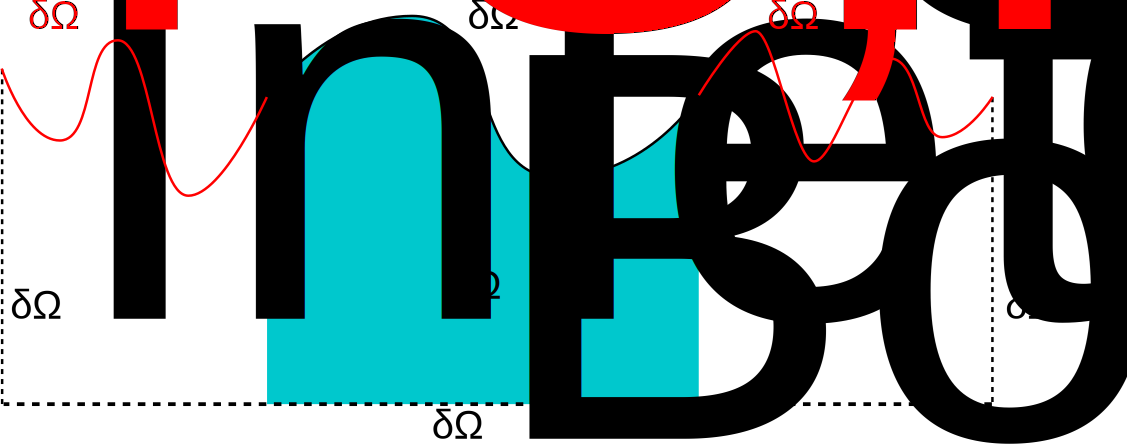
\includegraphics[width=0.6\textwidth]{Omega2}
  \caption{Computational domain $\Omega$}
  \label{fig:ss:laplace3D:bem}
\end{figure}
%
\subsection{Boundary conditions (BC)}
\label{sss:laplace3D:BC}
%
In order to can purpose an evolution process we need to use
the boundary conditions along the free surface. In the most
general way we can rewrite the Bernoulli equation, that is
the dynamic free surface boundary condition (DFSBC), as (see
\citep{yang2004}):
%
\begin{eqnarray}
	\label{eq:laplace3D:FS_Bernoulli}
	\frac{\mbox{D} \phi(x,y,z;t)}{\mbox{D} t} =
		\frac{1}{2}\left\vert \gradient \phi \right\vert^2
		- g z(x,y;t)
		- \frac{p_0}{\rho}
		- \bs{U}(t) \cdot \gradient \phi(x,y,z;t)
		- \frac{\partial \bs{U}(t)}{\partial t} \cdot (x,y,0)
\end{eqnarray}
%
Where $p_0$ is the atmospheric pressure, that we will consider
null, and $\bs{U}(t)$ is the ship velocity, in this case will be
a null vector. Since the material derivative denotes
%
\begin{eqnarray*}
	\frac{\mbox{D} f}{\mbox{D} t} =
		\frac{\partial f}{\partial t}
		\gradient{\phi(x,y,z;t)} \cdot \gradient{f}
\end{eqnarray*}
%
We can rewrite the dynamic boundary condition for this specific case as
%
\begin{eqnarray}
	\label{eq:laplace3D:DFSBC}
	\frac{\partial \phi(x,y,z;t)}{\partial t} =
		- \frac{1}{2}\left\vert \gradient \phi \right\vert^2
		- g z(x,y;t)
\end{eqnarray}
%
Regarding the kinematic free surface boundary condition (KFSBC), in the
most general way we can write that
%
\begin{eqnarray}
	\label{eq:laplace3D:FS_Kinematic}
	\frac{\mbox{D} z(x,y;t)}{\mbox{D} t} =
		\frac{\partial \phi(x,y,z;t)}{\partial z}
		- \bs{U}(t) \cdot \gradient z(x,y;t)
\end{eqnarray}
%
Where we can expand the material derivative, writing the KFSBC for this
specific case
%
\begin{eqnarray}
	\label{eq:laplace3D:KFSBC}
	\frac{\partial z(x,y;t)}{\partial t} =
		\frac{\partial \phi(x,y,z;t)}{\partial z}
		- \gradient{\phi(x,y,z;t)} \cdot \gradient{z(x,y;t)}
\end{eqnarray}
%
\subsection{Time integration scheme}
\label{sss:laplace3D:TimeIntegration}
%
We may start the simulation in a initial condition where we know the
full free surface shape and velocity potential, including the gradients.
%
\begin{eqnarray}
	\label{eq:laplace3D:IC}
	\begin{array}{lcl}
		z(x,y;t=0) & = & z_0(x,y)
		\\
		\phi(x,y,z;t=0) & = & \phi_0(x,y,z)
		\\
		\gradient z(x,y;t=0) & = & \gradient z_0(x,y)
		\\
		\gradient \phi(x,y,z;t=0) & = & \gradient \phi_0(x,y,z)
	\end{array}
\end{eqnarray}
%
In the computational part of the free surface is enough to know the free
surface shape $z_0(x,y)$ and the velocity potential $\phi_0(x,y,z)$.\rc
%
For simplicity we will use an Euler's integration scheme, but the same
method can be easily applied for any other explicit time integrator, like
the Adams-Bashforth ones.\rc
%
In each time step we start knowing the shape of the free surface, and the
velocity potential, and basically we want to compute these fields for the
next time step. To do it the following steps are followed:
%
\begin{enumerate}
	\item We use BEM to compute the velocity potential gradient, as will be
	described in the section \ref{sss:laplace3D:bem_solve}.
	\begin{eqnarray}
		\label{eq:laplace3D:time_march:bem}
		\gradient{\phi(x,y,z;t)} = \mbox{BEM}\left(\phi(x,y,z;t), z(x,y;t)\right)
	\end{eqnarray}
	\item We use the KFSBC to compute the derivative of the free surface
	elevation, and the DFSBC to know the derivative of the velocity potential.
	\begin{eqnarray}
		\label{eq:laplace3D:time_march:dzdt}
		\frac{\partial z(x,y;t)}{\partial t} = &
			\mbox{KFSBC}\left(\gradient{\phi(x,y,z;t)}\right)
		\\
		\label{eq:laplace3D:time_march:dphidt}
		\frac{\partial \phi(x,y,z;t)}{\partial t} = &
			\mbox{DFSBC}\left(z(x,y;t), \gradient{\phi(x,y,z;t)}\right)
	\end{eqnarray}
	\item And then we can perform the time integration.
	\begin{eqnarray}
		\label{eq:laplace3D:time_march:z_integrate}
		z(x,y;t + \Delta t) = &
			z(x,y;t) +
			\Delta t \dsty \frac{\partial z(x,y;t)}{\partial t}
		\\
		\label{eq:laplace3D:time_march:phi_integrate}
		\phi(x,y,z;t + \Delta t) = &
			\phi(x,y,z;t + \Delta t) +
			\Delta t \dsty \frac{\partial \phi(x,y,z;t)}{\partial t}
	\end{eqnarray}
\end{enumerate}
%
\subsection{Discrete Laplace solution using the BEM}
\label{sss:laplace3D:bem_solve}
%
As we have seen in the previous sections we want to use the BEM in order
to compute the velocity potential gradient in the free surface from the
velocity potential value known. In the equation
\ref{eq:laplace3D:reciprocal_relation} we can starting dividing the domain
contour as shown in the figure \ref{fig:ss:laplace3D:bem}, getting the
computational one, denoted by $\partial \Omega_{FS}$, and
the extension one, denoted by $\partial \Omega_{FS,I}$, where the free
surface and the velocity potential and gradient is known for all the
time instants.
%
\begin{eqnarray}
	\label{eq:laplace3D:reciprocal_relation:002}
	\begin{array}{l}
	\frac{1}{2} \phi(X, Y, Z; t) =
	\\
	\dsty \int_{\partial \Omega_{FS}}
		\phi(x, y, z; t) \frac{\partial G(x, y, z, X, Y, Z)}{\partial \bs{n}(x, y, z)} -
		G(x, y, z, X, Y, Z) \frac{\partial \phi(x, y, z; t)}{\partial \bs{n}(x, y, z)}
		\mbox{d} s(x, y, z)
	\\
	\dsty \int_{\partial \Omega_{FS,I}}
		\phi(x, y, z; t) \frac{\partial G(x, y, z, X, Y, Z)}{\partial \bs{n}(x, y, z)} -
		G(x, y, z, X, Y, Z) \frac{\partial \phi(x, y, z; t)}{\partial \bs{n}(x, y, z)}
		\mbox{d} s(x, y, z)		
	\end{array}
\end{eqnarray}
%
Where we already assumed that $(x,y,z) \in \partial \Omega$. We can start discretizing
the velocity potential, assuming that the potential and their gradient changes smoothly
enough. The our contours can be divided according to the grid:
%
\begin{eqnarray}
	\label{eq:laplace3D:reciprocal_relation:003}
	\begin{array}{rl}
	\frac{1}{2} \phi_a = &
	\dsty \sum_{b=1}^{n_{FS}}
		\phi_b
		\dsty \int_{\partial \Omega_{FS}^b} H(\bs{x}, \bs{x}_a) \mbox{d} s(\bs{x})
	-
	\dsty \sum_{b=1}^{n_{FS}}
		\frac{\partial \phi_b}{\partial \bs{n}_b}
		\dsty \int_{\partial \Omega_{FS}^b} G(\bs{x}, \bs{x}_a) \mbox{d} s(\bs{x})
	\\
	&
	\dsty \sum_{b=1}^{n_{FS,I}}
		\phi_b
		\dsty \int_{\partial \Omega_{FS,I}^b} H(\bs{x}, \bs{x}_a) \mbox{d} s(\bs{x})
	-
	\dsty \sum_{b=1}^{n_{FS,I}}
		\frac{\partial \phi_b}{\partial \bs{n}_b}
		\dsty \int_{\partial \Omega_{FS,I}^b} G(\bs{x}, \bs{x}_a) \mbox{d} s(\bs{x})
	\end{array}
\end{eqnarray}
%
The functions $G(x,y,z,X,Y,Z)$ and $H(x,y,z,X,Y,Z)$, according to the equations
\ref{eq:laplace3D:g} and \ref{eq:laplace3D:h}, are well defined in all the
subintervals where $(x,y,z) \neq (X,Y,Z)$, and are so quite smooth, so we will
change all the integrals that accomplish it for point evaluations.
%
\begin{eqnarray}
	\label{eq:laplace3D:reciprocal_relation:004}
	\begin{array}{rl}
	\frac{1}{2} \phi_a = &
		\phi_a
		\dsty \int_{\partial \Omega_{FS}^a} H(\bs{x}, \bs{x}_a) \mbox{d} s(\bs{x})
	-
		\frac{\partial \phi_a}{\partial \bs{n}_a}
		\dsty \int_{\partial \Omega_{FS}^a} G(\bs{x}, \bs{x}_a) \mbox{d} s(\bs{x})
	\\
	&
	\dsty \sum_{\substack{b = 1 \\ b \neq a}}^{n_{FS}}
	\left(
		\phi_b H_{ba} - \frac{\partial \phi_b}{\partial \bs{n}_b} G_{ba}
	\right) S_b
	+
	\dsty \sum_{b=1}^{n_{FS,I}}
	\left(
		\phi_b H_{ba} - \frac{\partial \phi_b}{\partial \bs{n}_b} G_{ba}
	\right) S_b
	\end{array}
\end{eqnarray}
%
The remaining integrals must be treated carefully since the functions are
singular in the center of the interval. $H(x,y,z,X,Y,Z)$ is an odd function,
so the limit of the integral when the radius of the interval goes to zero
is null, being well defined. Regarding the function $G(x,y,z,X,Y,Z)$ is an
even function of order:
%
\begin{eqnarray*}
	G(\bs{x},\bs{x_a}) = \mathcal{O}\left(\frac{1}{\vert \bs{x} - \bs{x_a}\vert}\right)
\end{eqnarray*}
%
Which their integral is defined if the function $z(x,y)$ is well defined
as well. So the remaining integrals can be numerically computed, being mindful
that:
%
\begin{enumerate}
	\item Can't be evaluated at the point $\bs{x_a}$.
	\item Changes too fast around the point $\bs{x_a}$.
\end{enumerate}
%
We will discuss later how to solve this integrals, for the moment we will define
new functions such that:
%
\begin{eqnarray}
	\label{eq:laplace3D:g:hat}
	\hat G_{ab} = 
	\left\lbrace \begin{array}{l}
		\dsty \int_{\partial \Omega_{FS}^a} G(\bs{x}, \bs{x}_a) \mbox{d} s(\bs{x}); \, \, \mbox{if} \, a = b
		\\
		G(\bs{x_b},\bs{x_a}) S_b; \, \, \mbox{if} \, a \neq b
	\end{array} \right.
	\\
	\label{eq:laplace3D:h:hat}
	\hat H_{ab} = 
	\left\lbrace \begin{array}{l}
		\dsty \int_{\partial \Omega_{FS}^a} H(\bs{x}, \bs{x}_a) \mbox{d} s(\bs{x}); \, \, \mbox{if} \, a = b
		\\
		H(\bs{x_b},\bs{x_a}) S_b; \, \, \mbox{if} \, a \neq b
	\end{array} \right.
\end{eqnarray}
%
So we can rewrite the equation \ref{eq:laplace3D:reciprocal_relation:004}
%
\begin{eqnarray}
	\label{eq:laplace3D:reciprocal_relation:005}
	\frac{1}{2} \phi_a
	=
	\dsty \sum_{b=1}^{n_{FS}}
	\left(
		\phi_b \hat H_{ba} - \frac{\partial \phi_b}{\partial \bs{n}_b} \hat G_{ba}
	\right)
	+
	\dsty \sum_{b=1}^{n_{FS,I}}
	\left(
		\phi_b \hat H_{ba} - \frac{\partial \phi_b}{\partial \bs{n}_b} \hat G_{ba}
	\right)
\end{eqnarray}
%
Where we can move all the terms of the computational free surface that affects
to the gradient of the velocity potential (that is the value that we want to
compute) to left hand side, and let all the other ones in the right hand side
of the equation
%
\begin{eqnarray}
	\label{eq:laplace3D:reciprocal_relation:006}
	\dsty \sum_{b \in \partial \Omega_{FS}}
		\frac{\partial \phi_b}{\partial \bs{n}_b} \hat G_{ba}
	=
	-
	\frac{1}{2} \phi_a
	+
	\dsty \sum_{b \in \partial \Omega_{FS}}
		\phi_b \hat H_{ba}
	+
	\dsty \sum_{b \in \partial \Omega_{FS,I}}
		\left(
		\phi_b \hat H_{ba} -
		\frac{\partial \phi_b}{\partial \bs{n}_b} \hat G_{ba} 
		\right)
\end{eqnarray}
%
The equation \ref{eq:laplace3D:reciprocal_relation:006}, that
has been written for the velocity potential at one point $\bs{x}_a$,
can be written for all the points of the free surface along
the computational domain using the matrix notation
%
\begin{eqnarray}
	\label{eq:laplace3D:reciprocal_relation:007}
	\mathcal{G} \left[ \frac{ \partial \phi}{\partial \bs{n}} \right]
	=
	\left( \mathcal{H} - \frac{1}{2} \mathcal{I} \right) \left[ \phi \right]
	+
	\mathcal{H}_{FS,I} \left[ \phi \right]_{FS,I}
	-
	\mathcal{G}_{FS,I} \left[ \frac{ \partial \phi}{\partial \bs{n}} \right]_{FS,I}
\end{eqnarray}
%
Note that the area of the elements $S_b$ has been included into
the matrices. The equation
\ref{eq:laplace3D:reciprocal_relation:007} is a linear system
of equations that can be numerically solved, either inverting
the matrix, or using an iterative method. The matrix inversion
is probably the best way for linear seakeeping codes, where the
same matrix will be ever used, but in this case the iterative
method is the faster way.\rc
%
The method described along this section allows to us to compute
the gradient of the velocity potential along the free surface
knowing the potential in the computational free surface, and both
velocity potential and the gradient along the extended free
surface.
%
\subsection{Integrals computation}
\label{sss:laplace3D:integrals}
%
In the equations \ref{eq:laplace3D:g:hat} and \ref{eq:laplace3D:g:hat}
we have introduced two inconvenient integrals. Even though the functions
are not well defined when $\bs{x} = \bs{x_a}$, their integrals it is.
For instance, if we can assume that the free surface is fully planar
($z = 0$), the integrals can be analytically computed
%
\begin{eqnarray*}
	\dsty \int_{y_a - \delta y}^{y_a + \delta y} \int_{x_a - \delta x}^{x_a + \delta x}
		G(x,y,0,x_a,y_a,0)
	\, \mbox{d}x \, \mbox{d}y
	= &
	\dsty \frac{
		\delta x \, \, \mbox{asinh}\left(\frac{\delta y}{\delta x}\right)
		+
		\delta y \, \, \mbox{asinh}\left(\frac{\delta x}{\delta y}\right)
	}{\pi}
	\\
	\dsty \int_{y_a - \delta y}^{y_a + \delta y} \int_{x_a - \delta x}^{x_a + \delta x}
		H(x,y,0,x_a,y_a,0)
	\, \mbox{d}x \, \mbox{d}y
	= &
	0
\end{eqnarray*}
%
But can not be analytically computed for every function $z(x,y)$, being
necessary to compute it in a numerical way.\rc
%
In the figure \ref{fig:ss:laplace3D:integral} a schematic representation
of the integration method is shown. Let we want to compute the integral
for an element of the grid $(x_a,y_a)$, then we subdivide the element in
\textbf{a even number} of subelements of area $dx \cdot dy$, so we can
assert that any subelement will be evaluated in the point $(x_a,y_a)$,
but as near as we want because we can ever add more subelements; then we
can numerically approximate the integral by (here in after we will use
only the function $G(\bs{x}, bs{x_a})$, because same method can be applied
to the function $H(\bs{x}, bs{x_a})$).
%
\begin{eqnarray}
	\label{eq:laplace3D:integral:g}
	\dsty \int_{\partial \Omega_{FS}^a} G(\bs{x}, \bs{x}_a) \mbox{d} s(\bs{x})
	\simeq
	\sum_{i=1}^{n_x} \sum_{j=1}^{n_y} G(x_i,y_j,z(x_i,y_i), x_a, y_a, z(x_a, y_a)) \, dx \, dy
\end{eqnarray}
%
Of course the value $z(x_a, y_a)$ is known, but not the function $z(x_i,y_i)$
because is evaluated in points that are not reflected in the grid, so we must
compute this points from the available data. We will start renormalizing the
coordinates such that:
%
\begin{eqnarray}
	\label{eq:laplace3D:integral:uv}
	\begin{array}{lcl}
	u & = & \dsty \frac{x - \left(x_a - Dx\right)}{2 Dx}
	\\
	v & = & \dsty \frac{y - \left(y_a - Dy\right)}{2 Dy} 
	\end{array}
\end{eqnarray}
%
So we know the value of $z$ for all the combinations of $u = 0,0.5,1$ and
$v = 0,0.5,1$. Then, to can evaluate the function $z(u,v)$ for all $u,v$
values we may to build a Spline surface with the data known from the 9
points shown in the figure \ref{fig:ss:laplace3D:integral}. The Spline
surface can be characterized as
%
\begin{eqnarray}
	\label{eq:laplace3D:integral:spline}
	z(u,v) = k_0 + k_u u + k_v v + k_{uv} u v + k_{uu} u^2 + k_{vv} v^2
	+ k_{uuv} u^2 v + k_{uvv} u v^2 + k_{uuvv} u^2 v^2
\end{eqnarray}
%
In the equation \ref{eq:laplace3D:integral:spline} we have 9 unknown
coefficients, but we have available $z(u,v)$ for 9 points, so have 9
unknowns with 9 equations that can be set as a linear system of
equations, that results in the following coefficients:
%
\begin{eqnarray}
	\label{eq:laplace3D:integral:k}
	\begin{array}{lcl}
	k_0 & = & z \left( 0,0 \right)
	\\
	k_u & = & - z \left( 1,0 \right) + 4 z \left( \frac{1}{2},0 \right) - 3 z \left( 0,0 \right)
	\\
	k_v & = & - z \left( 0,1 \right) + 4 z \left( 0,\frac{1}{2} \right) - 3 z \left( 0,0 \right)
	\\
	k_{uv} & = & z \left( 1,1 \right) - 4 z \left( 1,\frac{1}{2} \right) + 3 z \left( 1,0 \right)
	             - 4 z \left( \frac{1}{2},1 \right) + 16 z \left( \frac{1}{2},\frac{1}{2} \right)
	        \\ & & 
	             - 12 z \left( \frac{1}{2},0 \right) + 3 z \left( 0,1 \right)
	             - 12 z \left( 0,\frac{1}{2} \right) + 9 z \left( 0,0 \right)
	\\
	k_{uu} & = & 2 z \left( 1,0 \right) - 4 z \left( \frac{1}{2},0 \right) + 2 z \left( 1,0 \right)
	\\
	k_{vv} & = & 2 z \left( 0,1 \right) - 4 z \left( 0,\frac{1}{2} \right) + 2 z \left( 1,0 \right)
	\\
	k_{uuv} & = & - 2 z \left( 1,1 \right) + 8 z \left( 1,\frac{1}{2} \right) - 6 z \left( 1,0 \right)
	              + 4 z \left( \frac{1}{2},1 \right) - 16 z \left( \frac{1}{2},\frac{1}{2} \right)
	        \\ & & 
	              + 12 z \left( \frac{1}{2},0 \right) - 2 z \left( 0,1 \right)
	              + 8 z \left( 0,\frac{1}{2} \right) - 6 z \left( 0,0 \right)
	\\
	k_{uvv} & = & - 2 z \left( 1,1 \right) + 4 z \left( 1,\frac{1}{2} \right) - 2 z \left( 1,0 \right)
	              + 8 z \left( \frac{1}{2},1 \right) - 16 z \left( \frac{1}{2},\frac{1}{2} \right)
	        \\ & & 
	              + 8 z \left( \frac{1}{2},0 \right) - 6 z \left( 0,1 \right)
	              + 12 z \left( 0,\frac{1}{2} \right) - 6 z \left( 0,0 \right)
	\\
	k_{uuvv} & = & 4 z \left( 1,1 \right) - 8 z \left( 1,\frac{1}{2} \right) + 4 z \left( 1,0 \right)
	               - 8 z \left( \frac{1}{2},1 \right) + 16 z \left( \frac{1}{2},\frac{1}{2} \right)
	        \\ & & 
	               - 8 z \left( \frac{1}{2},0 \right) + 4 z \left( 0,1 \right)
	               - 8 z \left( 0,\frac{1}{2} \right) + 4 z \left( 0,0 \right)
	\end{array}
\end{eqnarray}
%
So using the equation \ref{eq:laplace3D:integral:g} to \ref{eq:laplace3D:integral:k}
we can compute the integrals in the equations \ref{eq:laplace3D:g:hat} and
\ref{eq:laplace3D:h:hat}.
%
\begin{figure}[ht!]
  \centering
  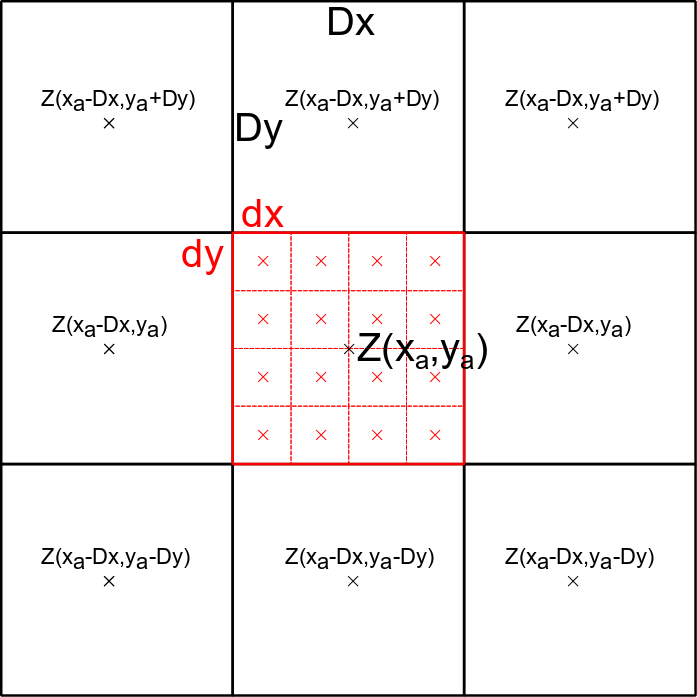
\includegraphics[width=0.6\textwidth]{Integral}
  \caption{Integration method scheme}
  \label{fig:ss:laplace3D:integral}
\end{figure}
%
\section{BEM test}
\label{ss:laplace3D:test}
%
\subsection{General}
\label{sss:laplace3D:test:general}
%
A Python script has been provided with this document in the subfolder \textbf{test}.
In the script  all this theory is tested in order to know if the BEM is well purposed,
and the errors that can be expected from the method application.\rc
%
In the test, for the moment, only one wave will be set, and the computational free
surface will be big enough to contain 2 wave lengths. In this case a wave period
of $T = 2.5 s$ is used, resulting in a wave of 10 meters.\rc
%
In the figure \ref{fig:laplace3D:test:wave} the wave used, that runs in the x direction,
is shown. The free surface will be extended while $G(x,y,z,X,Y,Z) > 0.1$.
%
\begin{figure}[ht!]
  \centering
  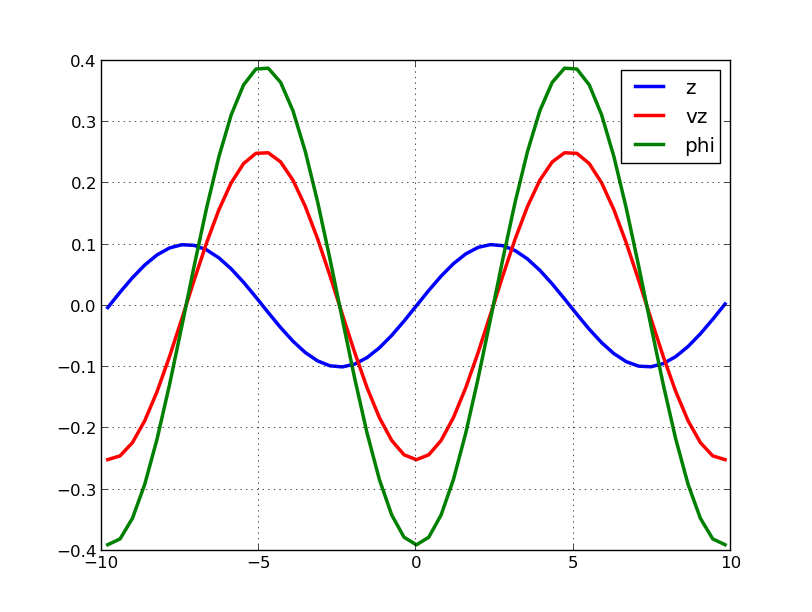
\includegraphics[width=0.6\textwidth]{test_wave}
  \caption{Wave used in the test}
  \label{fig:laplace3D:test:wave}
\end{figure}
%
\subsection{Direct method}
\label{sss:laplace3D:test:direct}
%
The direct method consist in evaluate the velocity potential in several points
using the equation \ref{eq:laplace3D:reciprocal_relation:005}, testing the error
get.\rc
%
If we apply the direct method for all the points of the computational free surface,
we can compute the root mean square error as
%
\begin{eqnarray*}
	RMS(nx,ny) = \sqrt{\frac{1}{nx \, ny} \sum_{i=1}^{nx} \sum_{j=1}^{ny}
		\left( \phi_{direct}(x_i,y_j) - \phi(x_i,y_j) \right)^2
	}
\end{eqnarray*}
%
For $nx = 31$ and $ny = 15$ we have $RMS(31,15) = 0.08$. In the figure
\ref{fig:laplace3D:test:direct} the analytic velocity potential, and the
interpolated using the direct method, for a slice in the middle of the
free surface ($y=0$).\rc
%
The results quality is good, and can be improved increasing the number of
points in the computational free surface.
%
\begin{figure}[ht!]
  \centering
  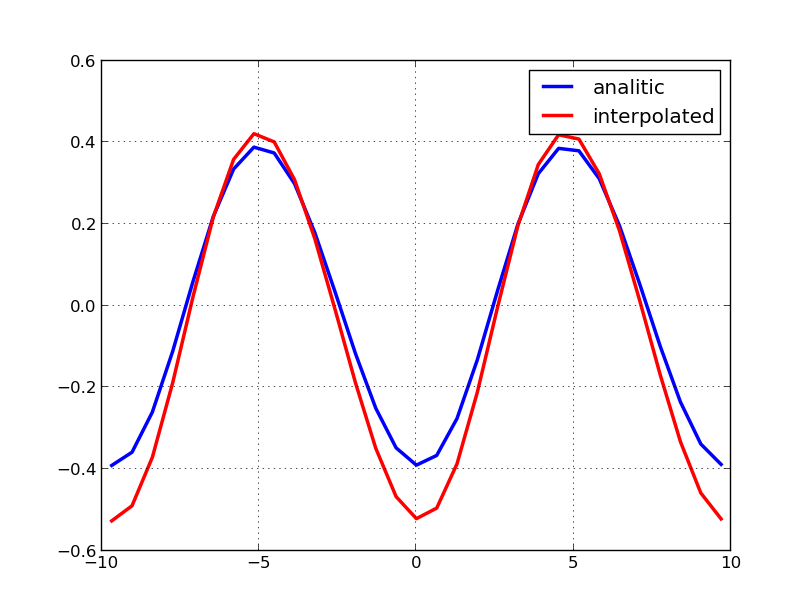
\includegraphics[width=0.6\textwidth]{test_direct}
  \caption{Direct method}
  \label{fig:laplace3D:test:direct}
\end{figure}
%
\subsection{BEM}
\label{sss:laplace3D:test:bem}
%
In this case we want to apply the equation \ref{eq:laplace3D:reciprocal_relation:006},
where a linear system of equations is purposed in order to compute the gradient of the
velocity potential, projected over the normal, for all the points of the grid.
%
For $nx = 31$ and $ny = 15$ we have $RMS(31,15) = 0.04$. In the figure
\ref{fig:laplace3D:test:bem} the analytic velocity potential, and the
interpolated using the direct method, for a slice in the middle of the
free surface ($y=0$).\rc
%
The results quality is nice like in the direct method. In order to get enough good
results at least 15 points per wave length must be used (like in this application).
%
\begin{figure}[ht!]
  \centering
  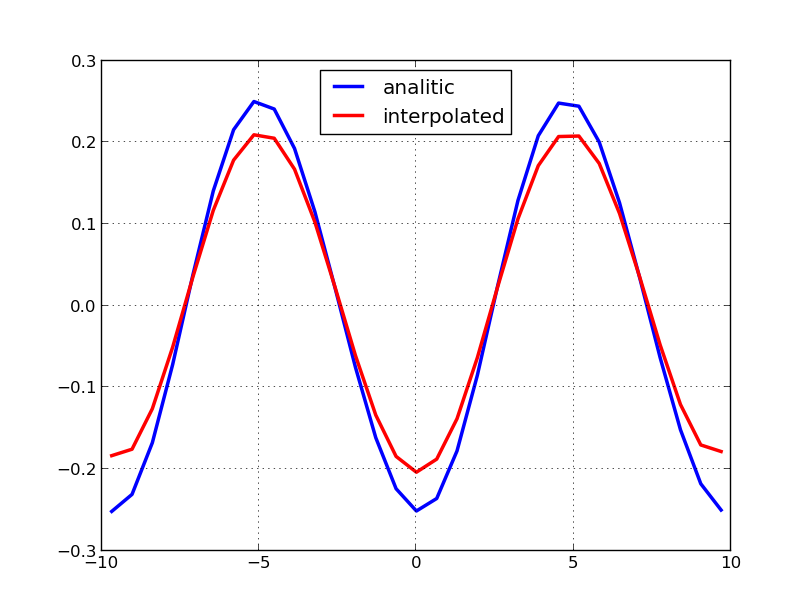
\includegraphics[width=0.6\textwidth]{test_bem}
  \caption{BEM solution}
  \label{fig:laplace3D:test:bem}
\end{figure}
%